%% LyX 2.3.0 created this file.  For more info, see http://www.lyx.org/.
%% Do not edit unless you really know what you are doing.
\documentclass[oneside,english]{amsart}
\usepackage[T1]{fontenc}
\usepackage[latin9]{inputenc}
\usepackage{geometry}
\geometry{verbose}
\setlength{\parskip}{\smallskipamount}
\setlength{\parindent}{0pt}
\synctex=-1
\usepackage{float}
\usepackage{url}
\usepackage{amsbsy}
\usepackage{amstext}
\usepackage{amsthm}
\usepackage{amssymb}
\usepackage{graphicx}
\usepackage[authoryear]{natbib}

\makeatletter

%%%%%%%%%%%%%%%%%%%%%%%%%%%%%% LyX specific LaTeX commands.
%% Because html converters don't know tabularnewline
\providecommand{\tabularnewline}{\\}
\floatstyle{ruled}
\newfloat{algorithm}{tbp}{loa}
\providecommand{\algorithmname}{Algorithm}
\floatname{algorithm}{\protect\algorithmname}

%%%%%%%%%%%%%%%%%%%%%%%%%%%%%% Textclass specific LaTeX commands.
\numberwithin{equation}{section}
\numberwithin{figure}{section}

%%%%%%%%%%%%%%%%%%%%%%%%%%%%%% User specified LaTeX commands.
\usepackage{tikz}
\usepackage{tikz-3dplot}
\usetikzlibrary{patterns}
\usetikzlibrary{matrix}
\usetikzlibrary{decorations.pathmorphing}
\usetikzlibrary{decorations.pathreplacing}
\usetikzlibrary{decorations.markings}
\usetikzlibrary{decorations.shapes}
\usetikzlibrary{arrows}
\usepackage{pgfplots}
\pgfplotsset{compat=newest}

\makeatother

\usepackage{babel}

\begin{document}

\title{Optimization of a discontinuous finite element solver with OpenCL
and StarPU}

\author{Philippe Helluy, Michel Massaro, Laura Mendoza, Bruno Weber}

\address{Universit� de Strasbourg, Inria Tonus, AxesSim. \texttt{philippe.helluy@unistra.fr}}
\begin{abstract}
\texttt{schnaps} is a finite element solver designed to simulate various
physical phenomena. It is designed to run on hybrid computers made
of several CPUs and GPUs. In order to address the hybrid architectures
we rely on the StarPU runtime. StarPU allows to optimize in an incremental
way a sequential algorithm in order to migrate to multicore parallelism
and then to hybrid computing with OpenCL accelerators. StarPU proposes
several task scheduling strategies in order to efficiently exploit the
available computing power. We present the design of \texttt{schnaps}
and the performance gain that we have obtained in electromagnetic
simulations thanks to OpenCL codelets.
\end{abstract}

\maketitle

\section{Introduction}

The development of engineering simulation software is difficult. On
one hand, the user is interested in handling more and more complex
physical phenomena, in devices with arbitrary geometries. These constraints
require to adopt a generic and abstract software engineering approach
in order to ensure the generality of the code. On the other hand,
the user also wants to harness the full computational power of his
hybrid computer. This requirement generally imposes to use low
level hardware optimization hacks that are not always compatible with
a generic and elegant approach. In addition, as the hardware evolves,
optimizations of yesterday are not necessarily relevant for the devices
of tomorrow...

OpenCL is a nice software environment for optimization purposes. It
presents the good balance between an abstract view of the computing
devices and some important hardware aspects, such as local memory
for accelerating data transfers or subgroups for minimizing synchronization
barriers. However depending on architecture, optimizations written
for one accelerator may be completely irrelevant for another one.
This is especially true with local memory optimizations. For instance,
cache prefetching is generally efficient for discrete GPUs while inefficient
for IGPs.

In this paper, we present our practical approach to this issue, with
the help of the StarPU runtime system. StarPU is developed at Inria
Bordeaux since 2006\footnote{We are not involved in the creation and development of StarPU, but
only users.}. 
StarPU is a runtime C library based on the dataflow paradigm. The
programmer has to split the computation workload into abstract computational
tasks. Each task processes data buffers that can be in \texttt{read} (R), \texttt{write}
(W) or \texttt{read/write} (RW) mode. 

The tasks are then conveniently implemented into C \emph{codelets}.
It is possible (and recommended) to write several implementations
of the same task into several codelets. For instance, one can imagine
to write an unoptimized codelet for validation purposes and one or
several optimized OpenCL codelets. The user then submits his
tasks in a sequential way to StarPU. At runtime, StarPU is able
to construct a task graph based on buffer dependencies. The tasks
are submitted to the available accelerators, in parallel if the dependencies
allow it. 
In addition, StarPU automatically handles data transfers between the
accelerators. It is also able to measure the efficiency of the different
codelets' implementations in order to choose the best, according to
the scheduling strategy. 

With StarPU, implementing a complex dataflow of OpenCL kernels becomes
easier. Indeed, the programmer does not have to handle the kernel
dependencies with OpenCL events. In addition, it is possible to first
write a well validated pure C version of the software, with only C
codelets. Then, one can enrich the tasks with OpenCL codelets, which
allows an incremental optimization of the code. At each stage, StarPU
should be able to use the available codelets in an efficient way.

In this paper, we describe how we applied the StarPU philosophy in order to optimize
a discontinuous finite element solver for conservation laws. The outlines
are as follows: first we will present in its main lines the Discontinuous
Galerkin (DG) scheme that is used in the solver. Then, after a short
presentation of StarPU, we will explain how we have integrated the
OpenCL optimizations into the DG solver. Finally, we will present
some numerical experiments.

\section{Discontinuous Galerkin method}

\global\long\def\vf{\mathbf{{f}}}
\global\long\def\vg{\mathbf{{g}}}
\global\long\def\vh{\mathbf{{h}}}
\global\long\def\vs{\mathbf{{s}}}
\global\long\def\vV{\mathbf{V}}
\global\long\def\vx{\mathbf{x}}
\global\long\def\v#1{\mathbf{#1}}
\global\long\def\vq{\mathbf{q}}
\global\long\def\vw{\mathbf{w}}
\global\long\def\ddim{D}
\global\long\def\dorder{d}
\global\long\def\normal{\mathbf{n}}
\global\long\def\flux{\mathbf{q}}
\global\long\def\Vu{\mathbf{u}}
\global\long\def\Vvi{\mathbf{v}_{i}}

The Discontinuous Galerkin (DG) method is a general finite element
method for approximating systems of conservation laws of the form
\[
\partial_{t}\v w+\sum_{k=1}^{\ddim}\partial_{k}\v f^{k}(\v w)=0.
\]
The unknown is the vector of conservative variables $\v w(\v x,t)\in\mathbb{R}^{m}$
depending on the space variable $\v x=(x^{1},\ldots,x^{\ddim})\in\mathbb{R}^{\ddim}$
and on time $t$. In this paper, the space dimension is $\ddim=3$. 
We adopt the notations $\partial_{t}$ for the partial derivative
with respect to $t$ and $\partial_{k}$ for the the partial derivative
with respect to $x^{k}$. Let $\v n=(n_{1},\ldots,n_{\ddim})\in\mathbb{R}^{\ddim}$
be a spatial direction, the flux in direction $\v n$ is defined by
\[
\v f(\v w,\v n)=\sum_{k=1}^{\ddim}n_{k}\v f^{k}(\v w).
\]
For instance in this work we consider the numerical simulation of
an electromagnetic wave. In this particular case, the conservative
variables are
\[
\v w=(\v E^\mathrm{T},\v H^\mathrm{T},\lambda,\mu)^\mathrm{T}\in\mathbb{R}^{m},\quad m=8.
\]
where $\v E\in\mathbb{R}^{3}$ is the electric field, $\v H\in\mathbb{R}^{3}$
is the magnetic field and $\lambda$, $\mu$ are divergence cleaning
potentials (\citet{munz2000divergence}). The flux is given by
\[
\v f(\v w,\v n)=\left(\begin{array}{c}
-\v n\times\v H+\lambda\v n\\
\v n\times\v E+\mu\v n\\
c\v n\cdot\v E\\
c\v{n\cdot H}
\end{array}\right)
\]
and $c>1$ is the divergence cleaning parameter.

We consider a mesh $\mathcal{M}$ of $\Omega$ made of open sets,
called \emph{cells}, $\mathcal{M}=\left\{ L_{i},\,i=1\ldots N_{c}\right\} $.
In the most general setting, the cells satisfy
\begin{enumerate}
\item $L_{i}\cap L_{j}=\emptyset$, if $i\neq j$;
\item $\overline{\cup_{i}L_{i}}=\overline{\Omega}.$
\end{enumerate}
In each cell $L\in\mathcal{M}$, we consider a basis of functions
$(\varphi_{L,i}(\vx))_{i=0\ldots N_{\dorder}-1}$ constructed from
polynomials of order $\dorder$.  We denote by $h$ the maximal diameter
of the cells. With an abuse of notation we still denote by $\vw$
the approximation of $\vw$, defined by
\[
\vw(\vx,t)=\sum_{j=0}^{N_{\dorder}-1}\vw_{L,j}(t)\varphi_{L,j}(\vx),\quad\vx\in L.
\]
The DG formulation then reads: find $\vw_{L,j}$ such that
for all cell $L$ and all test function $\varphi_{L,i}$
\begin{equation}
\int_{L}\partial_{t}\vw_{L}\varphi_{L,i}-\int_{L}\vf(\vw_{L},\boldsymbol{\nabla}\varphi_{L,i})+\int_{\partial L}\vf(\vw_{L},\vw_{R},\v n)\varphi_{L,i}=0.\label{eq:dg_var}
\end{equation}
In this formula (see Figure \ref{fig:cell_convention}):
\begin{itemize}
\item $R$ denotes the neighboring cell to $L$ along its boundary $\partial L\cap\partial R$,
or the exterior of $\Omega$ on $\partial L\cap\partial\Omega$.
\item $\normal=\normal_{LR}$ is the unit normal vector on $\partial L$
oriented from $L$ to $R$.
\item $\vw_{R}$ denotes the value of $\vw$ in the neighboring cell $R$
on $\partial L\cap\partial R$.
\item If $L$ is a boundary cell, one may have to use the boundary values
instead: $\vw_{R}=\vw_{b}$ on $\partial L\cap\partial\Omega$.
\item $\vf(\vw_{L},\vw_{R},\v n)$ is the standard upwind numerical flux
encountered in many finite volume or DG methods.
\end{itemize}
\begin{figure}
\begin{centering}
\begin{center}
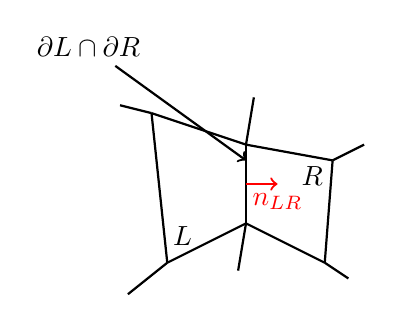
\begin{tikzpicture}[scale=1]
% intersection 
\draw[thick] (0,1) -- (0,0); \draw[->, thick, color=red] (0,0.5) -- (0.4,0.5); \node[below, color=red] at (0.4,0.5) {$n_{LR}$}; \node[above] (n1) at (-2,2) {$\partial L\cap\partial R$}; \draw[->, thick] (n1) -- (0,0.8);
% left  
\draw[thick] (-1,-0.5) -- (0,0); \draw[thick] (-1.2,1.4) -- (0,1); \draw[thick] (-1.2,1.4) -- (-1,-0.5); \node[above right] at (-1.05,-0.4) {$L$}; 
% right  
\draw[thick] (1,-0.5) -- (0,0); \draw[thick] (1.1,0.8) -- (0,1); \draw[thick] (1.1,0.8) -- (1,-0.5); \node[below left] at (1.1,0.85) {$R$};
% other quadrangles
\draw[thick] (0,0) -- (-0.1,-0.6); \draw[thick] (0,1) -- (0.1,1.6); \draw[thick] (-1,-0.5) -- (-1.5,-0.9); \draw[thick] (-1.2,1.4) -- (-1.6,1.5); \draw[thick] (1,-0.5) -- (1.3,-0.7); \draw[thick] (1.1,0.8) -- (1.5,1);  \end{tikzpicture} 
\par\end{center}
\par\end{centering}
\caption{\label{fig:cell_convention}Convention for the $L$ and $R$ cells
orientation.}
\end{figure}

In our application, we consider hexahedral cells. We have a reference
cell 
\[
\hat{L}=]-1,1[^{\ddim}
\]
\global\long\def\jacob{\boldsymbol{\tau}}
and a smooth transformation $\vx=\jacob_{L}(\hat{\vx})$, $\hat{\vx}\in\hat{L}$,
that maps $\hat{L}$ on $L$
\[
\jacob_{L}(\hat{L})=L.
\]
We assume that $\jacob_{L}$ is invertible and we denote by $\jacob_{L}'$
its (invertible) Jacobian matrix. We also assume that $\jacob_{L}$
is a direct transformation
\[
\det\jacob_{L}'>0.
\]
In our implementation, $\jacob_{L}$ is a quadratic map based on hexahedral
curved ``H20'' finite elements with 20 nodes. The mesh of H20 finite
elements is generated by \texttt{gmsh} (\citet{geuzaine2009gmsh}). 

On the reference cell, we consider the Gauss-Lobatto points $(\hat{\vx}_{i})_{i=0\ldots N_{\dorder}-1}$,
$N_{\dorder}=(\dorder+1)^{\ddim}$ and associated weights $(\omega_{i})_{i=0\ldots N_{\dorder}-1}$.
They are obtained by tensor products of the $(\dorder+1)$ one-dimensional
Gauss-Lobatto (GL) points on $]-1,1[$. The reference GL points and
weights are then mapped to the physical GL points of cell $L$ by
\begin{equation}
\vx_{L,i}=\jacob_{L}(\hat{\vx}_{i}),\quad\omega_{L,i}=\omega_{i}\det\jacob_{L}'(\hat{\vx}_{i})>0.\label{eq:map_GL}
\end{equation}
In addition, the six faces of the reference hexahedral cell are denoted
by $F_{\epsilon}$, $\epsilon=1\ldots6$ and the corresponding outward
normal vectors are denoted by $\hat{\normal}_{\epsilon}$. One advantage
of choosing the GL points is that the cells and the faces share the
same quadrature points. We use the following notations to define
the face quadrature weights:
\begin{itemize}
\item if a GL point $\hat{\vx}_{i}\in F_{\epsilon}$, we denote by $\mu_{i}^{\epsilon}$
the corresponding quadrature weight on face $\vw_{\epsilon}$;
\item we also use the convention that $\mu_{i}^{\epsilon}=0$ if $\hat{\vx}_{i}$
does not belong to face $F_{\epsilon}$.
\end{itemize}
Let us remark that a given GL point $\hat{\vx}_{i}$ can belong to
several faces when it is on an edge or in a corner of $\hat{L}$.
Because of symmetry, we observe that if $\mu_{i}^{\epsilon}\neq0$,
then the weight $\mu_{i}^{\epsilon}$ does not depend on $\epsilon$.

We then consider basis functions $\hat{\varphi_{i}}$ on the reference
cell: they are the Lagrange polynomials associated to the Gauss-Lobatto
points and thus satisfy the interpolation property
\[
\hat{\varphi}_{i}(\hat{\vx}_{j})=\delta_{ij}.
\]
The basis functions on cell $L$ are then defined according to the
formula
\[
\varphi_{L,i}(\vx)=\hat{\varphi}_{i}(\jacob_{L}^{-1}(\vx)).
\]
In this way, they also satisfy the interpolation property
\begin{equation}
\varphi_{L,i}(\vx_{L,j})=\delta_{ij}.\label{eq:interp_property}
\end{equation}
In this paper, we only consider conformal meshes: the GL points on
cell $L$ are supposed to match the GL points of cell $R$ on their
common face. Dealing with non-matching cells is the object of a forthcoming
work.
Let $L$ and $R$ be two neighboring cells. Let $\vx_{L,j}$ be a
GL point in cell $L$ that is also on the common face between $L$
and $R$. In the case of conformal meshes, it is possible to define
the index $j'$ such that
\[
\vx_{L,j}=\vx_{R,j'}.
\]
 

Applying a numerical integration to (\ref{eq:dg_var}), using (\ref{eq:map_GL})
and the interpolation property (\ref{eq:interp_property}), we finally
obtain
\begin{equation}
\partial_{t}\vw_{L,i}\omega_{L,i}-\sum_{j=0}^{N_{\dorder}-1}\vf(\vw_{L,j},\boldsymbol{\nabla}\varphi_{L,i}(\vx_{L,j}))\omega_{L,j}+
\sum_{\epsilon=1}^{6}\mu_{i}^{\epsilon}\vf(\vw_{L,i},\vw_{R,i'},\normal_{\epsilon}(\vx_{L,i}))=0.\label{eq:dg_lobatto}
\end{equation}
We have to detail how the gradients and normal vectors are computed
in the above formula. Let $\v A$ be a square matrix. We recall that
the cofactor matrix of $\v A$ is defined by
\begin{equation}
\text{co}(\v A)=\det(\v A)\left(\v A^{-1}\right)^\mathrm{T}.\label{eq:co_mat}
\end{equation}
The gradient of the basis function is computed from the gradients
on the reference cell using (\ref{eq:co_mat})
\[
\boldsymbol{\nabla}\varphi_{L,i}(\vx_{L,j})=\frac{1}{\det\jacob_{L}'(\hat{\vx}_{j})}\text{co}(\jacob_{L}'(\hat{\vx}_{j}))\hat{\nabla}\hat{\varphi}_{i}(\hat{\vx}_{j}).
\]
In the same way, the scaled normal vectors $\v n_{\epsilon}$ on the
faces are computed by the formula
\[
\normal_{\epsilon}(\vx_{L,i})=\text{co}(\jacob_{L}'(\hat{\vx}_{i}))\hat{\normal}_{\epsilon}.
\]
We introduce the following notation for the cofactor matrix\global\long\def\comat{\mathbf{c}}
\[
\comat_{L,i}=\text{co}(\jacob_{L}'(\hat{\vx}_{i})).
\]
The DG scheme then reads
\begin{equation}
\partial_{t}\vw_{L,i}-\frac{1}{\omega_{L,i}}\sum_{j=0}^{N_{\dorder}-1}\vf(\vw_{L,j},\comat_{L,j}\hat{\nabla}\hat{\varphi}_{i}(\hat{\vx}_{j}))\omega_{j}+\frac{1}{\omega_{L,i}}\sum_{\epsilon=1}^{6}\mu_{i}^{\epsilon}\vf\left(\vw_{L,i},\vw_{R,i'},\comat_{L,i}\hat{\normal}_{\epsilon}\right)=0.\label{eq:DG_reduit}
\end{equation}

In formula (\ref{eq:DG_reduit}) we identify volume terms that are
associated to Gauss-Lobatto points in the volume
\begin{equation}
V_{i,j}=\vf(\vw_{L,j},\comat_{L,j}\hat{\nabla}\hat{\varphi}_{i}(\hat{\vx}_{j}))\omega_{j}\label{eq:volume_terms}
\end{equation}
and surface terms that are associated to cell boundaries
\begin{equation}
S_{i,i'}=\mu_{i}^{\epsilon}\vf\left(\vw_{L,i},\vw_{R,i'},\comat_{L,i}\hat{\normal}_{\epsilon}\right).\label{eq:surface_terms}
\end{equation}
Then, once these terms have been accumulated, one has to apply the
inverse of the mass matrix. Here, this matrix is diagonal and it corresponds
to a simple multiplication of $\partial_{t}\v w_{L,i}$ by
\begin{equation}
\frac{1}{\omega_{L,i}}.\label{eq:mass_matrix}
\end{equation}
Generally, $i$ and $i'$ are associated to unknowns of internal cells,
\emph{i.e.} cells that do not touch the boundaries. On boundary GL points,
the value of $\vw_{R,i'}$ is given by the boundary condition
\[
\vw_{R,i'}=\vw_{b}(\vx_{L,i},t),\quad\vx_{L,i}=\vx_{R,i'}.
\]
For practical reasons, it can be interesting to also consider $\vw_{R,i'}$
as an artificial unknown in a fictitious cell. The fictitious unknown
is then a solution of the differential equation
\begin{equation}
\partial_{t}\vw_{R,i'}=\partial_{t}\v w_{b}(\vx_{L,i},\cdot).\label{eq:fictitious_ODE}
\end{equation}
In the end, if we put all the unknowns in a large vector $\v W(t)$,
(\ref{eq:DG_reduit}) and (\ref{eq:fictitious_ODE}) read as a large
system of coupled differential equations
\begin{equation}
\partial_{t}\v W=\v F(\v W).\label{eq:linear_ODE}
\end{equation}
This set of differential equations is then numerically solved by a
Runge-Kutta numerical method. In practice, we use a second order Runge-Kutta
method (RK2).

\section{Data-based parallelism and StarPU}

StarPU is a runtime system library developed at Inria Bordeaux (\citet{augonnet2011starpu,augonnet2012starpu}).
It relies on the data-based parallelism paradigm.
The user has first to split its whole problem into elementary computational
tasks. The elementary tasks are then implemented into \emph{codelets},
which are simple C functions. The same task can be implemented differently
into several codelets. This allows the user to harness special accelerators,
such as vectorial CPU cores or OpenCL devices, for example.
In the StarPU terminology these devices are called \emph{workers}.
If a codelet contains OpenCL kernel submissions, special utilities
are available in order to map the StarPU buffers to OpenCL buffers.

For each task, the user also has to describe precisely what are the
input data, in \texttt{read} mode, and the output data, in \texttt{write}
or \texttt{read/write} mode. The user then submits the task in a sequential
way to the StarPU system. StarPU is able to construct at runtime a
task graph from the data dependencies. The task graph is analyzed
and the tasks are scheduled automatically to the available workers
(CPU cores, GPUs, \emph{etc}.). If possible, they are executed in
parallel into concurrent threads. The data transfer tasks between
the threads are automatically generated and managed by StarPU. OpenCL
data transfers are also managed by StarPU.

When a StarPU program is executed, it is possible to choose among
several schedulers. The simplest \texttt{eager} scheduler adopts a
very simple strategy: the tasks are executed in the order of
submission by the free workers, without optimization. More sophisticated
schedulers, such as the \texttt{dmda} or \texttt{dmdar} scheduler,
are able to measure the efficiency of the different codelets and the
data transfer times, in order to apply a more efficient allocation
of tasks.

Recently a new data access mode has been added to StarPU: the \texttt{commute}
mode. In a task, a buffer of data can now be accessed in \texttt{commute} mode,
in addition to the \texttt{write} or \texttt{read/write} modes. A \texttt{commute} access tells
to StarPU that the execution of the corresponding task may be executed
before or after other tasks containing commutative access. This allows
StarPU to perform additional optimizations.

There also exists a MPI version of StarPU. In the MPI version, the
user has to decide an initial distribution of data among the MPI nodes.
Then the tasks are submitted as usual (using the function starpu\_mpi\_insert\_task
instead of starpu\_insert\_task). Required MPI communications are
automatically generated by StarPU. For the moment, this approach does
not guarantee a good load balancing. It is the responsibility of the
user to migrate data from one MPI node to another to improve the
load balancing, if necessary. The MPI version of StarPU is not tested
in this work.

\subsection{\label{subsec:Macrocell-approach}Macrocell approach}

StarPU is quite efficient, but there is an unavoidable overhead due
to the task submissions and to the on-the-fly construction and analysis
of the task graph. Therefore it is important to ensure that the computational
tasks are not too small, in which case the overhead would not be amortized,
or not too big, in which case some workers would be idle.
To achieve the right balance, we decided not to apply the
DG algorithm at the cell level but to groups of cells instead.

The implementation of the DG scheme has been made into the \texttt{schnaps}
software\footnote{\url{http://schnaps.gforge.inria.fr/}}
which is a C99 software dedicated to the numerical simulation
of conservation laws. 
In \texttt{schnaps}, we first construct a \emph{macromesh} of the
computational domain. Then each \emph{macrocell} of the macromesh
is split into \emph{subcells}. See Figure \ref{fig:macrocell_mesh}. We also
arrange the subcells into a regular sub-mesh of the macrocells. In
this way, it is possible to apply additional optimizations. For instance,
the subcells $L$ of a same macrocell $\mathcal{L}$ share
the same geometrical transformation $\jacob_{L}$, which saves memory
access.

\begin{figure}
\begin{centering}
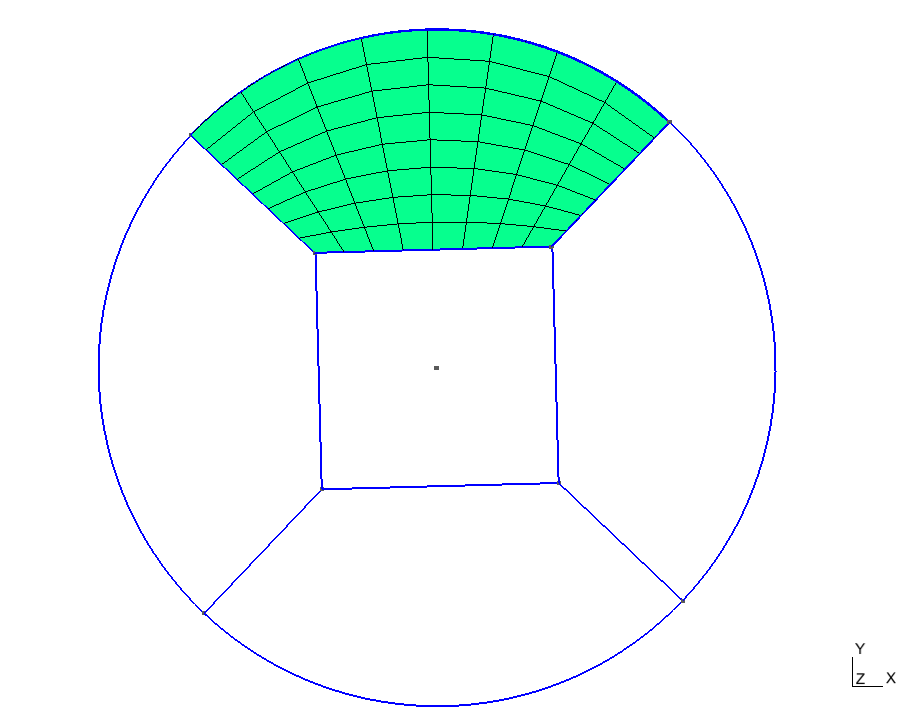
\includegraphics[height=6cm]{../../../kirsch/doc/CEMRACS16/img/lackdisque}
\par\end{centering}
\caption{\label{fig:macrocell_mesh}Macrocell approach: an example of a mesh
made of five macrocells. Each macrocell is then split into several
subcells. Only the subcells of the top macrocell are represented here
(in green).}
\end{figure}

In \texttt{schnaps} we also defined an \emph{interface} structure
in order to manage data communications between the macrocells. An
interface contains a copy of the data at the Gauss-Lobatto points
that are common to the two neighboring macrocells.

To solve one time step of the DG method, here are the most
important tasks:
\begin{enumerate}
\item Interface extraction: this task simply extracts the values of $\vw$
coming from the neighboring macrocells to the interface. In this task,
the macrocell buffers are accessed in \texttt{read} mode and the interface
data in \texttt{write} mode.
\item Interface fluxes: this task only computes the numerical fluxes (\ref{eq:surface_terms})
that are located at the Gauss-Lobatto points on the interface. The fluxes
are then applied to the neighboring macrocells. In this task, the
interface data are accessed in \texttt{read} mode and the macrocell data in
\texttt{read/write} mode. For a better efficiency, we also assume a \texttt{commute}
access to the macrocell data. In this way the interface fluxes can
be assembled in any order, which can help the StarPU scheduling.
\item Interface boundary fluxes: this task computes the boundary data and
only numerical fluxes (\ref{eq:surface_terms}) that are located at
the boundary interface. The fluxes are applied to the neighboring
macrocell. In this task, the interface data are accessed in \texttt{read} mode
and the macrocell data in \texttt{read/write} and \texttt{commute} mode.
\item Volume terms: this task applies the volumic terms (\ref{eq:volume_terms})
in a given macrocell. The macrocell data are accessed in \texttt{read/write/commute}
mode.
\item Subcell fluxes: this task applies the numerical subcell fluxes (\ref{eq:surface_terms})
that are internal to a given macrocell. The macrocell data are accessed
in \texttt{read/write/commute} mode.
\end{enumerate}
Additional simple tasks are needed to apply the Runge-Kutta algorithm.
We do not describe them.

\begin{algorithm}
for all interface:

Extract interface (copy the data from the neighboring macrocells to
the interface)

If the interface is a boundary interface, compute the boundary fluxes
(\ref{eq:surface_terms}) and apply them to the neighboring macrocell

Else the interface is an internal one. Compute the numerical fluxes
(\ref{eq:surface_terms}) and apply them to the two neighboring macrocells

End for

Then, for each macrocell:

Compute and apply the numerical fluxes (\ref{eq:surface_terms}) between
the subcells

Compute the volume terms (\ref{eq:volume_terms}) inside the subcells 

Apply the inverse of the mass matrix (\ref{eq:mass_matrix})
inside the subcells

End for

\caption{\label{alg:DG-algorithm}DG algorithm}

\end{algorithm}

The general sequential DG algorithm is then given in Algorithm \ref{alg:DG-algorithm}.
Thanks to StarPU, this algorithm can be submitted in a sequential
way. StarPU then uses the data dependency in order to distribute
the tasks in parallel on the available workers.

In the next section we give more details about the implementation
of the OpenCL codelets.

\section{\label{sec:Hybrid-C/OpenCL-codelets}Hybrid C/OpenCL codelets}

In order to attain better performance, we programmed an OpenCL
version of the previously described codelets. As it is often the case,
special care has to be given in order to improve the coalescence of
memory access. The values of $\v w$ at the Gauss-Lobatto points are
stored into what we call a \emph{field} structure. A field is attached
to a macrocell. A given component of $\v w$ in a field is located
thanks to its subcell index \texttt{ic}, a Gauss-Lobatto index \texttt{ig}
in the cell, and a component index \texttt{iw}. If the macrocell is
cut into $n_{r}$ subcells in each direction, if the polynomial order
is $d$ and for a system of $m$ conservation laws, these indices
have the following bounds
\[
0\leq\mathtt{ic}<n_{r}^{3},\quad0\leq\mathtt{ig}<(d+1)^{3},\quad0\leq\mathtt{iw}<m.
\]

The values of $\v w$ in a given field are stored into a memory buffer
\texttt{wbuf}. In order to test several memory arrangements, the index
in the buffer is computed by a function \texttt{varindex(ic,ig,iw)}
that we can easily change. For instance, we can consider the following formula,
in which the electromagnetic components at a given Gauss-Lobatto point
are grouped in memory
\begin{equation}
\mathtt{varindex(ic,ig,iw)=iw+}m\mathtt{*(ig+}(d+1)^{3}\mathtt{*ic)},\label{eq:by_comp}
\end{equation}
or this formula
\begin{equation}
\mathtt{varindex(ic,ig,iw)=ig+}(d+1)^{3}\mathtt{*(iw+}m\mathtt{*ic)},\label{eq:by_gauss_point}
\end{equation}
in which the electromagnetic components are separated in memory. We
have programmed an OpenCL codelet for each task described in Section
\ref{subsec:Macrocell-approach}. The most time consuming kernels
are: (i) the kernel associated to the computations of the volume terms
(\ref{eq:volume_terms}) inside the macrocells, \emph{volume} kernel,
and (ii) the kernel that computes the subcell fluxes, the \emph{surface}
kernel. Boundary and interface terms generally involve less
computations.

A natural distribution of the workload is to associate one subcell
to each OpenCL work-group and the computations at a Gauss point to
a work-item. With this natural distribution, formula (\ref{eq:by_gauss_point})
ensures optimal coalescent memory access in the volume kernel,
but the access is no more optimal in the surface kernel, because
neighboring Gauss points on the subcell interfaces are not necessarily
close in memory. Therefore, we prefer considering formula
(\ref{eq:by_comp}). 

\section{Numerical results}

In this section, we present some practical experiments that we
realized with \texttt{schnaps}. The first experiment deals with the efficiency
of the StarPU C99 codelets on a multicore CPU. The second experiment
deals with the efficiency of the OpenCL codelets. Then we test the
code in a CPU/GPU configuration.

We approximate by the DG algorithm an exact plane wave solution of
the Maxwell equations
\[
\v E=\frac{c}{r}\left(\begin{array}{c}
-v\\
u\\
0
\end{array}\right),\quad\v H=\frac{c}{r}\left(\begin{array}{c}
0\\
0\\
1
\end{array}\right),\quad\lambda=0,\quad\mu=0.
\]
with $c=-\cos(\pi/2(ux^{1}+vx^{2}-t))$ and $(u,v)=(\cos(\pi/4),\sin(\pi/4)).$ 

We consider the propagation of the previous electromagnetic plane
wave into a torus-shaped domain $\Omega$ represented on Figure \ref{fig:Computational-domain}.
In the DG solver, we consider only third order polynomials: $d=3$.
The domain is split into $M=400$ macrocells. The macrocells are split
into $n_{r}$ subcells in each direction. The number of degrees of
freedom is thus
\[
n_{\text{d.o.f.}}=Mm(d+1)^{3}n_{r}^{3},\quad M=400,\quad m=8,\quad d=3.
\]

StarPU will have to take decisions on how to distribute efficiently
the tasks on the available accelerators.
We have performed our experiments on two different computers. The
first configuration ``PC'' correspond to a standard desktop personnal
computer. The second configuration ``WS'' is made of a more powerful
two-CPU workstation The technical details are listed in Table \ref{tab:config_specs}.

\begin{table}

\begin{centering}
\resizebox{0.9\linewidth}{!}{%
\begin{tabular}{|c|c|c|c|c|c|}
\hline 
config. & CPU & \# cores & mem. CPU & GPU & mem. GPU\tabularnewline
\hline 
\hline 
``PC'' & {\small{}AMD FX-8320E 3.2 GHz} & 8 & 8 GB & {\small{}NVIDIA GTX 1050 Ti} & 4 GB\tabularnewline
\hline 
``WS'' & {\small{}Intel Xeon E5-2609 1.7 GHz} & 2$\times$8 & 64 GB & {\small{}NVIDIA QUADRO P6000} & 24 GB\tabularnewline
\hline 
\end{tabular}}\caption{\label{tab:config_specs}Configurations of the computers used for
the tests.}
\par\end{centering}
\end{table}


\subsection{Multicore CPU tests}

In the first test, we only activate the C99 codelets, and thus the
GPU is not activated. We also vary the number of computing CPU cores
from 2 to 7 for the ``PC'' configuration and from 2 to 15 for the
``WS'' configuration. One CPU core is anyway reserved for the main
StarPU thread.

We perform a fixed number of $n_{t}$ iterations of the RK2 algorithm.
We assume that the number of elementary computing operations increases
as $O(n_{r}^{3}).$ Ideally, with infinitely fast operations at interfaces,
and with $n_{a}$ identical CPU cores, the computations time would
behave like 
\begin{equation}
T\sim Cn_{t}\frac{n_{r}^{3}}{n_{a}}\label{eq:ideal_time}
\end{equation}
where $C$ is fixed constant, depending on the hardware. In our benchmark
the \emph{efficiency} is the ratio of the measured execution time over
this ideal time. Normally it should be smaller than one (because of
communications). If it is close to one, the algorithm is very efficient.
In Table \ref{tab:bench_pc_cpu} and \ref{tab:bench_ws_cpu}, we observe
an excellent efficiency of the StarPU task distribution on the CPU
cores even on a machine with two NUMA nodes.

\begin{table}
\begin{centering}
\begin{tabular}{|c|c|c|c|c|}
\hline 
$n_{r}$ & $n_{\text{cpu}}$ & Time (s) & Ideal time & Efficiency\tabularnewline
\hline 
\hline 
4 & 2 & 704 & 704 & 1\tabularnewline
\hline 
4 & 4 & 365 & 352 & 0.96\tabularnewline
\hline 
4 & 7 & 209 & 201 & 0.96\tabularnewline
\hline 
6 & 7 & 689 & 679 & 0.99\tabularnewline
\hline 
8 & 4 & 2902 & 2816 & 0.97\tabularnewline
\hline 
8 & 7 & 1650 & 1609 & 0.98\tabularnewline
\hline 
\end{tabular}\caption{\label{tab:bench_pc_cpu}Efficiency of the CPU codelets for the ``PC''
configuration with the \texttt{dmdar} scheduler.}
\par\end{centering}
\end{table}

\begin{table}
\centering{}%
\begin{tabular}{|c|c|c|c|c|}
\hline 
$n_{r}$ & $n_{\text{cpu}}$ & Time (s) & Ideal time & Efficiency\tabularnewline
\hline 
\hline 
4 & 2 & 763 & 763 & 1\tabularnewline
\hline 
4 & 4 & 382 & 381 & 0.99\tabularnewline
\hline 
4 & 8 & 196 & 191 & 0.97\tabularnewline
\hline 
4 & 15 & 110 & 102 & 0.92\tabularnewline
\hline 
8 & 8 & 1586 & 1526 & 0.96\tabularnewline
\hline 
8 & 15 & 828 & 814 & 0.98\tabularnewline
\hline 
\end{tabular}\caption{\label{tab:bench_ws_cpu}Efficiency of the CPU codelets for the ``WS''
configuration with the \texttt{dmdar} scheduler.}
\end{table}


\subsection{OpenCL codelets}
\begin{sloppypar}
In this section, we compare the efficiency of the CPU/C99 and GPU/OpenCL
codelets on the two configurations ``PC'' and ``WS''. We first
perform a CPU-only computation with all the cores activated (7 for
the ``PC'' platform and 15 for the ``WS'' platform) and a GPU-only
computation. The results are given in Table \ref{tab:bench_cpu_gpu}.
We observe that the OpenCL codelets are faster than the CPU codelets.
The highest efficiency is achieved for the finer meshes ($n_{r}=8$). 
\end{sloppypar}

\begin{table}
\centering{}%
\begin{tabular}{|c|c|c|c|c|c|c|}
\hline 
$n_{r}$ & config. & $t_{\text{CPU}}$ (s) & $t_{\text{GPU}}$(s) & $t_{\text{CPU}}/t_{\text{GPU}}$ & $t_{\text{CPU+GPU}}$ (s) & $t_{\text{CPU}}/t_{\text{CPU+GPU}}$\tabularnewline
\hline 
\hline 
4 & PC & 209 & 73 & 2.86 & 32 & 6.53\tabularnewline
\hline 
6 & PC & 689 & 86 & 8.01 & 64 & 10.77\tabularnewline
\hline 
8 & PC & 1650 & 171 & 9.65 & 130 & 12.69\tabularnewline
\hline 
4 & WS & 110 & 86 & 1.28 & 36 & 3.05\tabularnewline
\hline 
8 & WS & 828 & 88 & 9.41 & 77 & 10.75\tabularnewline
\hline 
\end{tabular}\caption{\label{tab:bench_cpu_gpu}Efficiency of the CPU/GPU implementation.}
\end{table}

\begin{figure}
\begin{centering}
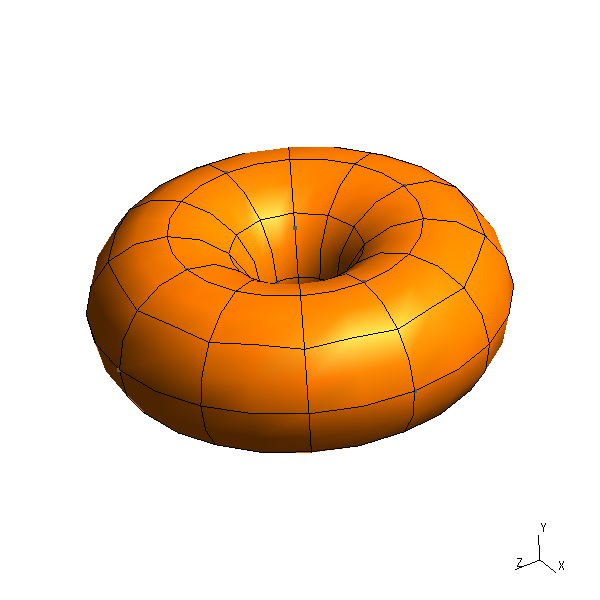
\includegraphics[width=6cm,trim={80 100 80 100},clip]{test_torus}
\par\end{centering}
\caption{\label{fig:Computational-domain}Computational domain $\Omega$. Only
the macrocells of the mesh are visible. The represented mesh contains
240 macrocells (poloidal refinement set to $n_{pol}=3$ and toroidal
refinement set to $n_{tor}=3$. In the numerical experiments, we take
$n_{pol}=3$ and $n_{tor}=5$, which leads to a mesh of 400 macrocells).
Each macrocell is then cut regularly into the three directions. }
\end{figure}


\subsection{Hybrid CPU/GPU computations}
\begin{sloppypar}
Now that we are equipped with verified OpenCL codelets we can try
to run the code with StarPU in order to see if it is able to distribute
the tasks efficiently on the available accelerators.
\end{sloppypar}

One difficulty is to manage efficiently the data transfers between
the accelerators. Several scheduling strategies are available in StarPU.
With the \texttt{eager} scheduler, the task are distributed in the order
of submission to the inactive device, without taking into account
the cost of memory transfers. This strategy is obviously not optimal.

It is better to choose another scheduler, such as the \texttt{dmdar}
scheduler. With the \texttt{dmdar} scheduler, the computational and memory
transfer costs are evaluated in a preliminary benchmarking phase.
Then an optimized scheduling is activated in order to better overlap
computations and communications.

We perform computations by letting StarPU decide how to distribute
the computations on the available CPU cores and GPU. 

The results are given in the two last columns of Table \ref{tab:bench_cpu_gpu}.
We observe that in all the situations, StarPU is able to get an additional
gain from the CPU cores, even if the GPU codelets are faster.

\section{Conclusion}

We have proposed an optimized implementation of the Discontinuous
Galerkin method on hybrid computer made of several GPUs and multicore
CPUs. In order to manage the heterogeneous architecture easily and
efficiently, we rely on OpenCL for the GPU computations and on the
StarPU runtime for distributing the computational tasks on the available
devices.

OpenCL programming becomes much easier because the task depndency
is computed by StarPU. We only had to concentrate on the optimization
of the individual OpenCL kernels and not on data distribution or
memory transfers. We first tested the efficiency of our OpenCL kernels.
We verified that the macrocell approach and cache prefetching strategy,
while not optiaml, give good results.

In addition, with a good choice of scheduler, and for heavy computations,
we have shown that StarPU is able to overlap computations and memory
transfer in a quite efficient way. It is also able to use
the available CPU codelts to achieve even higher acceleration.

\bibliographystyle{plainnat}
\bibliography{schnaps_opencl2017}


\end{document}
